\jxhj{%教学后记
	}
\skrq{%授课日期
	2017年9月12日 4-5节}
\ktmq{%课题名称
	基本指令及写程序思路 }
\jxmb{%教学目标,每行前面要加 \item
	\item 掌握手工编程的流程;
    \item 掌握基本指令;
    \item 编写矩形凸台的程序;
    \item 掌握编程基本思路。}
\jxzd{%教学重点,每行前面要加 \item
	\item 掌握G90、G91、G0、G1指令;
	\item 编写数控程序的基本思路;}
\jxnd{%教学难点,每行前面要加 \item
	\item 掌握G90、G91、G0、G1指令;}
\jjff{%教学方法
	通过讲述、举例、演示法来说明;}

\makeshouye %制作教案首页

%%%%教学内容
\subsection{组织教学}
\begin{enumerate}[1、]
	\item 集中学生注意力;
	\item 清查学生人数;
	\item 维持课堂纪律;
\end{enumerate}
\subsection{复习导入及主要内容}
\begin{enumerate}[1、]
    \item 数控编程的坐标系及假设;
    \item 数控程序的结构;
    \item 数控程序的指令;
    \item 数控编程的方式;
    \item 编写程序的基本思路。
\end{enumerate}
\subsection{教学内容及过程}
\subsubsection{案例分析}

在数控铣床或加工中心上加工如图\ref{fig:3-1}所示的零件,试完成程序的编写,已知毛坯为 $\Phi$ 110*30。

\begin{figure}
    \centering
    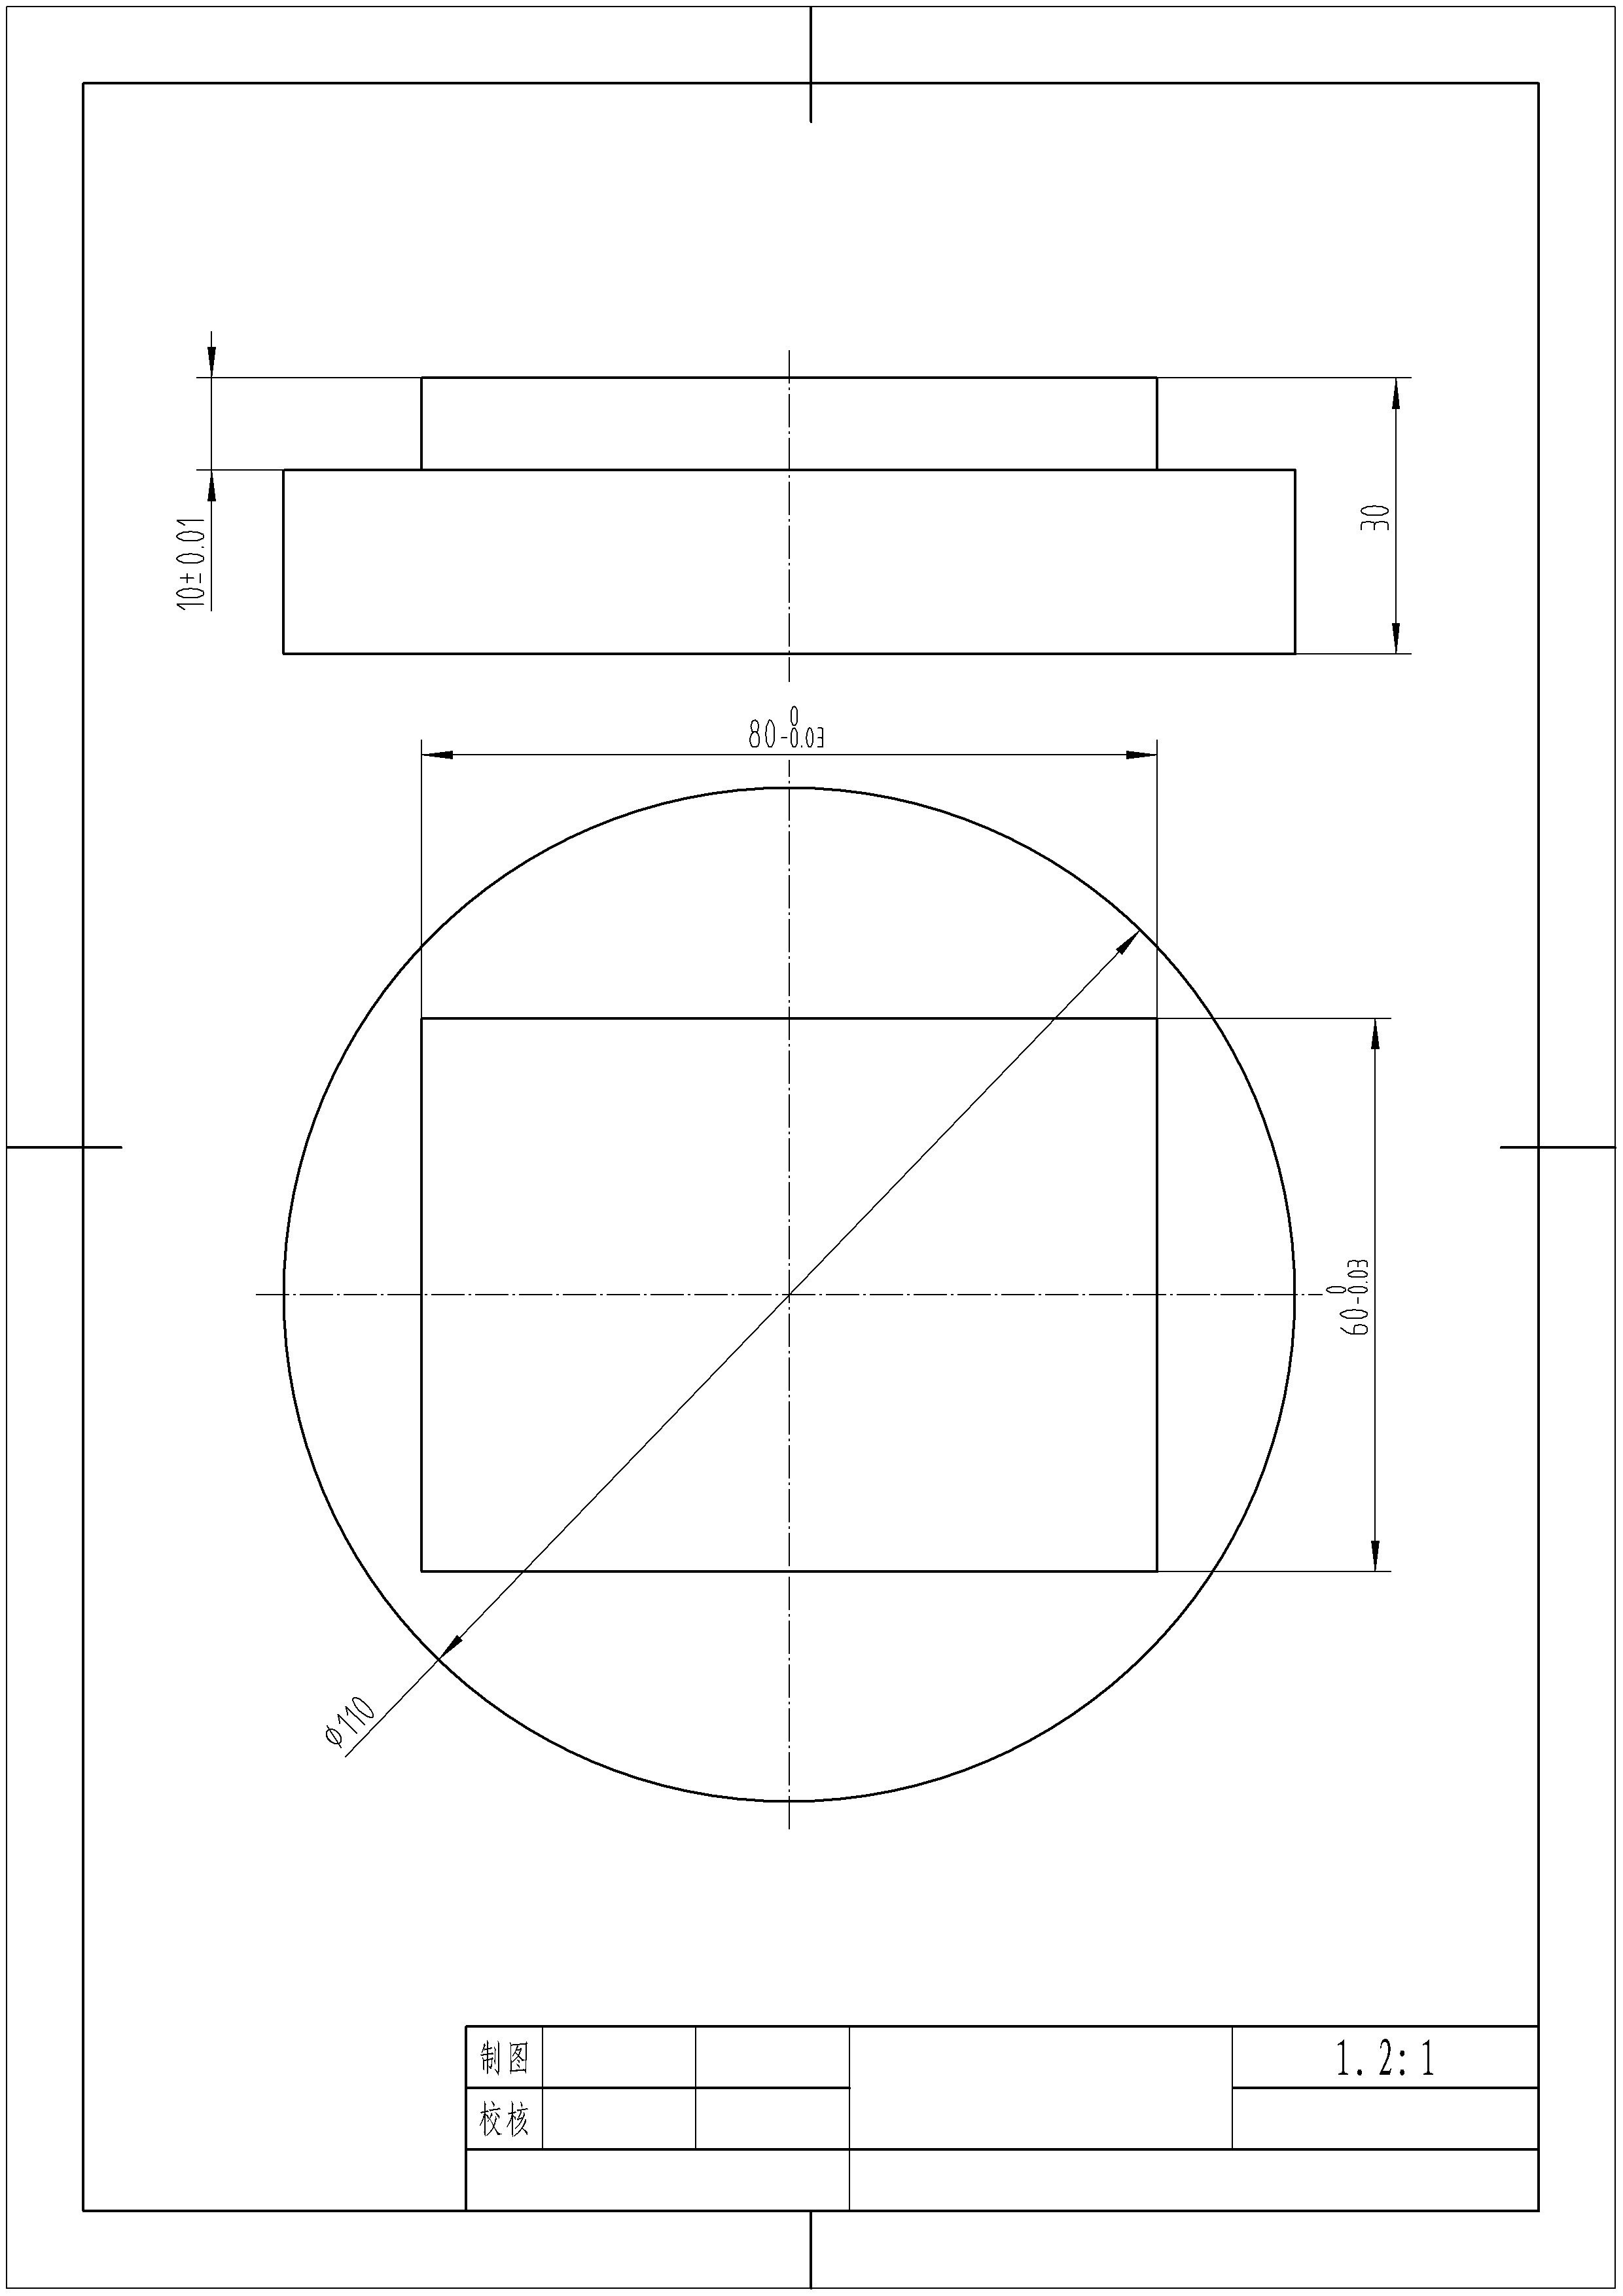
\includegraphics[width=0.8\linewidth,trim=50 150 50 100,clip]{data/image/3-1.jpg}
    \caption{}
    \label{fig:3-1}
\end{figure}

\begin{enumerate}[1、]
    \item 图样分析;
    \item 确定加工内容;
    \item 确定装夹及工件坐标系;
    \item 确定刀具及切削用量;
    \item 确定工序及走刀路线;
    \item 计算点坐标;
    \item 编写程序单。
\end{enumerate}

\subsubsection{程序名}
1、Fanuc的程序号与Siemens的程序名

Fanuc中用程序号区分各程序,程序号由位址O跟4位数字构成;是号,也就是说O0001号与O1号,表示同一个程序。

注意:1-7999为用户区域

8000-8999为加锁用户区域

9000-9999为厂方提供(扩展功能如O9001为换刀程序,也是加锁的)

所以用户最好别用8000-9999这些号码

2、Siemens中用程序名来区分各程序,确定程序名的规则是:

A、开始的两个符号必须是字母

B、其后的符号可以是字母,数字或下划线

C、最多为16个字符

D、不得使用分隔符

\subsubsection{安全注销指令}
1、G54-G59  选用工件坐标系,(后面讲)。

2、G17-G19  加工平面选择:

G17:XY平面 第一轴为X轴

G18:YZ平面 第一轴为Y轴

G19: ZX平面 第一轴为Z轴

圆弧指令、刀具半径补偿指令、钻孔指令等使用之前有设定平面。

3、G40、G49、G80 取消半径补偿、长度补偿、钻孔循环。

4、G90、G91 绝对坐标编程 增量坐标编程

G90指令按绝对坐标方式设定输入坐标,即移动指令终点的坐标值X、Y、Z都是以工件坐标系统坐标原点(程序零点)为基准来计算。

G91指令按增量坐标方式设定输入坐标,即移动指令终点的坐标值X、Y、Z都是以始点为基准来计算,再根据终点相对于始点的方向判断正负,与坐标轴正方向一致则取正,相反取负。

一般用G90,需要时采用G91,用完应立即改成G90。

\subsubsection{主轴正反转}
M3 S\verb|____| 主轴正转,其中S设定主轴转速,单位为r/min.

注意:本学校的机床,只有加工中心可以用S,数控铣床是机械调速,S无效,Siemens上不能使用S,不然机床会一直等主轴到达设定的转速后,才接着执行后面的程序。

\subsubsection{位移指令G0、G1}
定位(G0)

G00指令使刀具以绝对或相对指令快速移到工件系统指定的位置。在绝对指令状态下,编程端点的坐标值。在相对指令状态下编程中刀具移动的距离。

[ 格式 ]

G00 IP\_\_;

IP\_\_ :
对于绝对指令,端点的坐标值。对于相对指令,是指刀具移动的距离。

[ 说明 ]

刀具轨迹通常不是一条直线。

G00指令的快速移动速度是由参数No.1420由机床制造商来设定的。在实际执行G00时,刀具在单节的开始加速到预先指定的速度并在单节的结束减速。在确认到位后执行下一单节。到位的含义是指进给马达在指定的误差范围内。这个范围是由制造商在参数No.1826中设定的。

刀具沿直线移动。

[ 格式 ]

G01 IP\_\_ F\_\_ ;

IP\_\_ : 对于绝对指令,指端点的坐标,相对指令是指刀具移动的距离。

F\_\_ : 刀具进给的速度(进给率)

[ 说明 ]

刀具以指定的进给率F沿直线移动到指定的位置。

进给率F有效直到赋予新值,不需要在每个单节都指定。

F码指定的进给率是沿刀具轨迹测量的。

如果不指定F值,则认为进给率为零。

每个轴的进给率方向如下:

[ 限制 ]

G01 αα ββ γγ ζζ Ff  ;

α轴方向的进给率:Fα=α/L ×f

β轴方向的进给率:Fβ=β/L ×f

γ轴方向的进给率:Fγ=γ/L ×f

ζ轴方向的进给率:Fζ=ζ/L ×f

L2 = α2 + β2 + γ2 + ζ2

[ 举例 ]

■直线插补


\subsubsection{编写程序的基本思路}
程序初始化(安全保护)--------辅助准备(换刀,主轴启动,切削液开)--------定位到起刀点--------快速下刀--------工进下刀--------走加工轮廓--------提刀---------快速提刀到安全平面-------程序结束(换刀,主轴停止,切削液关,程序返回等)
\subsection{课堂小结}
\begin{enumerate}[1、]
\item 案例分析;
\item 指令讲解;
\item 编写程序;
\item 编写程序的基本思路。
\end{enumerate}
\vfill
\subsection{布置作业}
\begin{enumerate}[1、]
	\item 自定尺寸,编写加工一个矩形外形的程序?
\end{enumerate}
\vfill